\chapter{Future Directions and Closing Remarks }

\setcounter{table}{0}
\renewcommand{\thetable}{4.\arabic{table}}
\setcounter{figure}{0}
\renewcommand{\thefigure}{4.\arabic{figure}}


\section{Introduction}
	The Ubiquitin Proteasome System (UPS) plays a central role in protein degradation in all eukaryotes, and impacts almost all aspects of plant growth and development. The selective removal of key regulatory and aberrant proteins occurs via the covalent attachment of the polypeptide ubiquitin followed by degradation via the 26S proteasome.  This central enzymatic effector of the UPS is made up of two sup-particles, the regulatory particle (RP) responsible for recognizing and unfolding ubiquitylated substrates, and the core particle (CP) which degrades the unfolded protein. The bulk of my thesis has been spent analyzing the sub-particles of the 26S proteasome and their interacting proteins, with follow-up analyses characterizing the interaction network of several CP-specific proteins that may be involved in plant proteasome assembly. 
	
	In Chapter 2, I developed the first downstream label-free quantitative analysis tool for the Morpheus mass spectrometry search engine, Morpheus Spectral Counter (MSpC) \citep{gemperline16}. The goal was to use this software to perform analyses of the plant 26S proteasome complex with a focus on analyzing its isoform composition. The Morpheus search engine typically identifies a greater number of peptide spectral matches (PSMs), and is considerably faster than other search engines \citep{wenger13}. MSpC combined with Morpheus outperformed other spectral counting based measures in both speed and accuracy \citep{gemperline16}. MSpC implements the proven dNSAF algorithm that corrects for protein length and uniqueness \citep{zhang10}. The software maps Peptide-Spectral Matches (PSMs) to Protein groups and determines if they are distinct or shared, and then corrects the spectral counts based on protein length and total number of PSMs identified in an experiment. I was able to determine the relative incorporation level for most of the CP subunit isoforms, and these results matched previously published data that utilized UV-VIS quantitative methods coupled with top-down mass spectrometry \citep{gemperline16, russell13}. MSpC in combination with MS/MS analyses was also used in Chapter 3 to analyze native-PAGE slices of proteasome samples affinity purified from inhibitor-treated tissue.  MSpC comes with an easy to use graphic user interface and indeed, others have already started to use the software. 

	In Chapter 3, I developed an affinity purification of the RP based on two isoforms of RPT4, RPT4a and RPT4b. I identified all of the core 26S proteasome subunits and their isoforms in these affinity preparations, showing that this protocol was suitable for analysis of the plant RP.  These purifications coupled with a previously developed purification that targeted the CP enabled me to affinity-purify samples that were statistically enriched for either the RP or CP sub-complexes. LFQ-MS/MS of these CP and RP enriched samples, along with mock affinity controls, enabled me to confidently identify a suite of interacting proteins that were CP- and RP-specific.  The most abundant CP-associated proteins identified in our samples were putative assembly chaperones PBAC1-4, while the most abundant RP-associated proteins identified were putative RP assembly chaperones NAS2, NAS6, and HSM3. Taken together these data suggest that affinity preparations targeting the CP contain only mature RP, and affinity purifications targeting the RP contain only mature CP. 
	
	Next, I used a combination of yeast-two-hybrid and split-YFP approaches to build an interaction network involving a subset of the CP-specific putative assembly chaperones (PBAC1-4), showing similar interactions as observed between their mammalian and yeast orthologs. I also show that the novel plant, CP-specific interactor, PAP1, interacts with putative assembly chaperone PBAC1, suggesting that PAP1 may have a role in plant proteasome assembly.  Additionally, I also used native-PAGE coupled with MS/MS analyses to identify possible assembly intermediates of the 26S proteasome that contain these putataive, CP-specific chaperones and show that these proteins co-migrate with proteasome subunits. PBAC1-4, and PAP1 are found to associate with fractions containing mostly $\alpha$ subunits and the assembly chaperone UMP1; whereas only PBAC1, PBAC2, and PAP1 associate with more mature forms of the CP. These data suggest that PBAC3 and PBAC4 may be acting early in assembly, while PBAC1 and PBAC2 may be acting later. This is reminiscent to the role played by orthologous proteins in mammalian and yeast systems \citep{le07}. Taken together the analyses herein provide the first glimpse at plant proteasome assembly, and the likely players involved. Finally, I go on to show that there are very few, if any, differences in protein isoform composition between proteasomes affinity-purified with tagged RPT4a and RPT4b, suggesting that plants assemble their isoforms in a random fashion. 

\section{Future Directions}

\subsection{Proteasome Purifications}
	Now that I have developed an affinity purification strategy that is based on the RP base subunit RPT4, it may be useful to also develop an affinity purification that is based on an RP lid subunit. We now have tools in plants to affinity purify the CP via PAG1, and the RP-base via RPT4 through my work presented in Chapter 3; however, we have no tools that specifically target the plant RP-lid. Tools in yeast exist to affinity purify the CP via PRE1, the RP base via RPT1, and the RP lid via RPN11 \citep{leggett05, leggett02}. RP-lid affinity preparations of the yeast proteasome based on RPN11 were able to identify the de-ubiquitylating enzyme Ubp6, and an E3 ubiquitin ligase Hul5, which both have likely orthologs in \textit{Arabidopsis}. Unfortunately, to date, Hul5 has not been identified in plant preparations. While I have been able to identify a suite of RP interacting proteins including likely orthologs for the assembly chaperones NAS2, NAS6, and HSM3, there may be additional proteins that associate with the plant RP lid specifically. Affinity purifications based on the RPN5 subunit may be an attractive candidate to explore, as C-terminal tags with GFP have been used successfully in the past to rescue plants deficient in RPN5 \citep{book09, marshall15}. Unfortunately, structural studies of RP-lid subunits in yeast have suggested that the C-termini are essential for proper RP-lid assembly \citep{estrin13}. Therefore, an N-terminal tag may be more appropriate. I have already generated constructs that contain N-terminally FLAG-tagged variants of RPN5a, and RPN5b driven by their native promoters, that could be transformed into \textit{Arabidopsis}, and analyzed.  
In my RP-based affinity preparations, I failed to identify several proteins that likely help the plant complex process substrates including obvious plant orthologs of UCH37, and RPN13. In yeast, RPN13 acts in concert with UCH37 to appropriately process substrates, with RPN13 binding ubiquitin, and UCH37 de-ubiquitylating substrates \citep{husnjak08, jiao14}. RPN13 binds the proteasome subunit RPN2 in a highly labile and sub-stoichiometric association \citep{sakata12}. It may be reasonable to try cross-linking strategies coupled with MS/MS analyses to identify additional sub-stoichiometric and labile interactors of the plant proteasome.
  
\subsection{CP Assembly Chaperones}
	The most abundant CP-specific proteasome-associated proteins (PAPs) identified, PBAC1-4, may be orthologs of the mammalian assembly chaperones PAC1-4. We have evidence that these proteins associate with the proteasome and are CP-specific, as they are not identified in affinity purifications that target the RP via RPT4. These putative chaperones form an interaction network that is reminiscent of their yeast and mammalian counterparts, and are found in putative assembly intermediates. While we have indirect evidence for protein interactions through both yeast-two-hybrid and bimolecular fluorescent complementation analysis, direct, \textit{in vitro} binding assays should be performed to validate these indirect interactions. This would provide further support for these proteins forming an interaction network like their yeast and mammalian counterparts. \textit{In vitro} binding assays would require expression in heterologous systems such as \textit{E. coli}, and purification of these PBAC1-4 proteins. I have already generated expression vectors using two separate tags (6x histidine and glutathione-s-transferase (GST)), and performed some preliminary expression in \textit{E. coli} of PBAC1-3, and PAP1 (Figure \ref{fig:expression}). PBAC4 was also recently cloned into the same expression vectors, but its expression has not been tested.  If post-translational modifications of these chaperones are required for their interaction, this may be a potential problem with \textit{in vitro} binding assays, and would not be recapitulated in an \textit{E. Coli} recombinant expression system. Another potential issue with \textit{in vitro} expression is that others have reported that yeast Pba3 and Pba4 were completely insoluble unless co-expressed \citep{kusmierczyk08}, so an alternative expression system may be required such as the Duet expression system, to allow expression of both PBAC3 and PBAC4 at the same time \citep{scheich07}.  

\begin{FPfigure}[Figure \ref{fig:expression} \textit{caption follows on next page}]
	\centering
	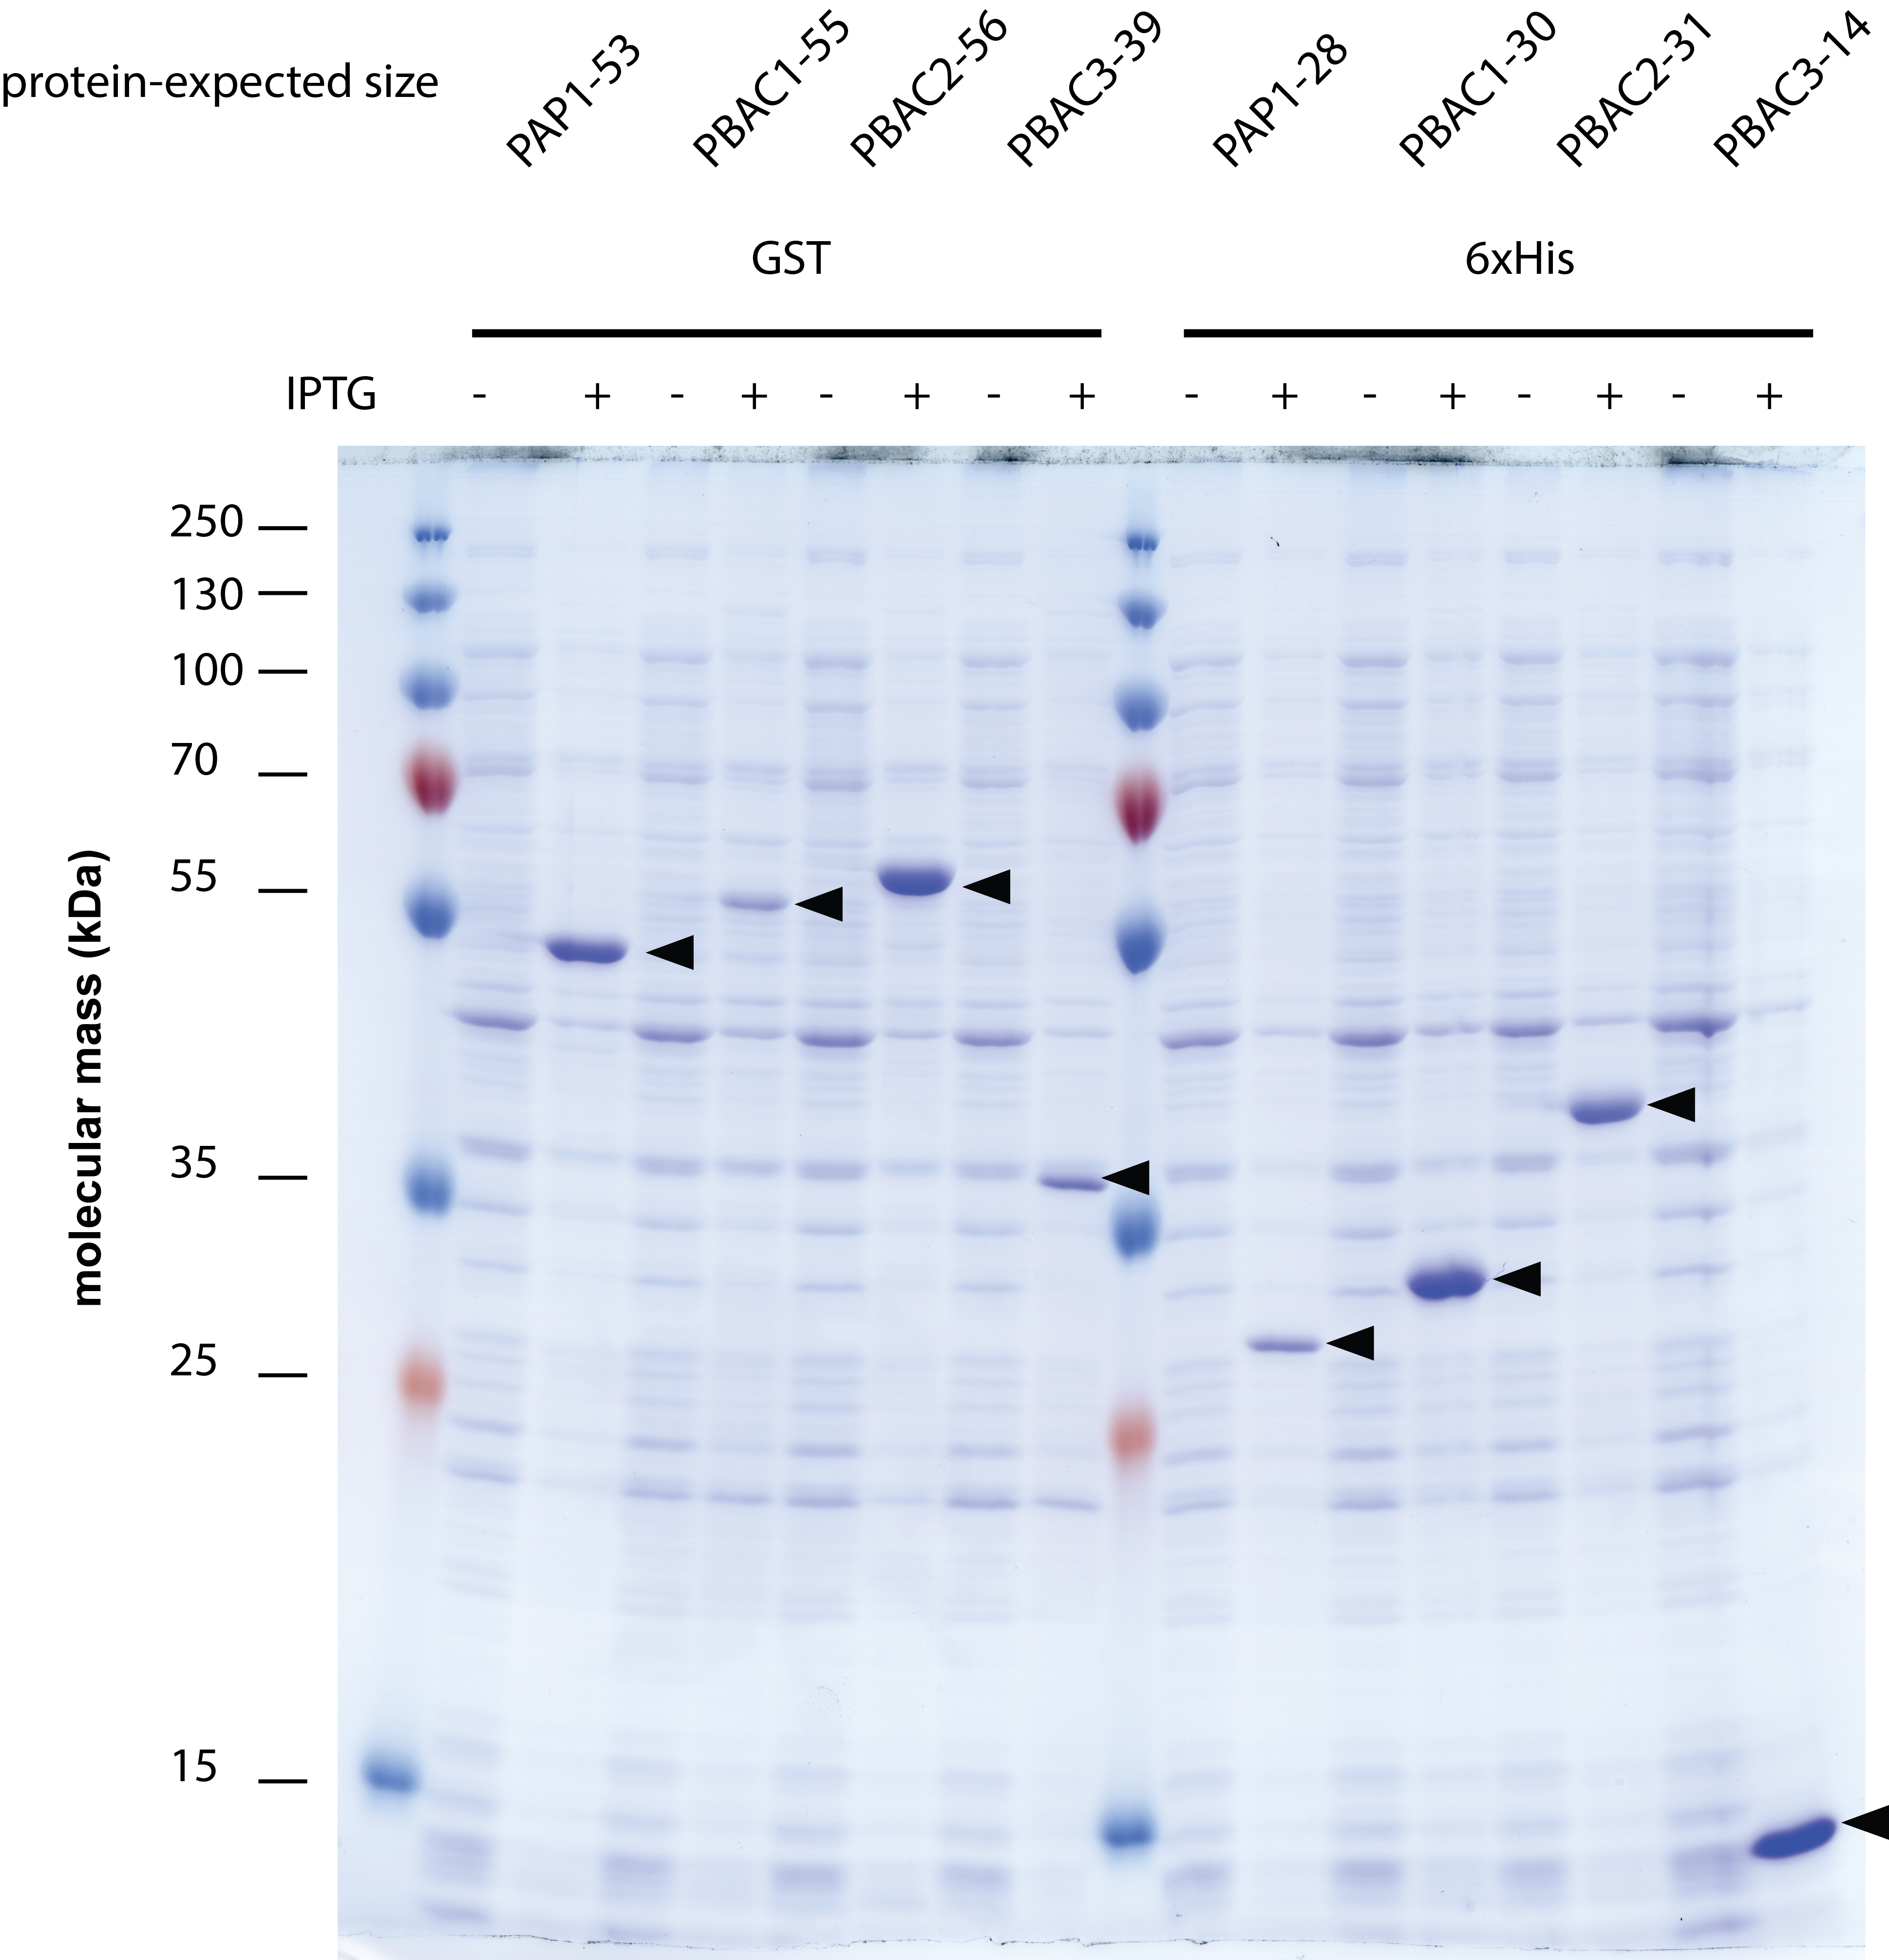
\includegraphics[width=\columnwidth]{future/expression.png}
	\mycaption{Recombinant protein expression of PAP1 and PBAC1-3}
	{Recombinant proteins were expressed in \textit{E. coli} BL21 DE3 with the indicated GST or 6xHis Tags. The corresponding protein extracts were then subjected to SDS-PAGE and then stained with Coomassie Blue. Protein extracts from IPTG-induced (+IPTG) and un-induced (-IPTG) control cultures are shown. At the top of each lane, samples are labeled with the name of the expressed protein followed by a number that defines the proteins expected size (in kDa). Black arrows on the gel indicate the likely induced proteins.}
	\label{fig:expression}
\end{FPfigure}
	
	Despite these downfalls, it would be useful to generate antibodies against PBAC1-4 as this would be helpful in determining the content of plant assembly intermediates. Assuming \textit{in vitro} expression of PBAC1-4 can be accomplished, these proteins (either expressed as heterodimeric pairs or alone) could also be used as bait to enrich for potential assembly intermediates from crude \textit{Arabidopsis} protein extracts. Proteins that interact with these bait proteins could then be determined by MS/MS analyses. 

	While PBAC1-4 associate with the CP and form an interaction network, it is unclear if these proteins function as assembly chaperones. Bioinformatic analyses, including PSI-BLAST and InterProScan domain analyses, are insufficient to determine that these proteins function as true CP assembly chaperones in plants. Analysis of \textit{Arabidopsis} plants deficient in \textit{PBAC1-4} will be useful in dissecting the plant proteasome assembly pathway.  I have not been able to confirm any mutants in \textit{PBAC1-4}; however, there may be candidates that could be tested (see Table \ref{table:tdna}). These genes are quite small, and identifying T-DNA insertions has proved challenging. A CRISPR based approach may be useful to precisely target these genes to generate single mutants, as well as combinations of mutants. 

\begin{table}[]
\centering
\mycaption{Candidate alleles for PBAC1-4}
{Candidate alleles were obtained from The Arabidopsis Information Resource \citep{berardini15} using T-DNA Express. SALK or SAIL identifiers are shown for PBAC1-4 with their predicted insertion sites.} 
\begingroup
\let\clearpage\relax
\scalebox{0.7}{
\begin{tabular}{@{}llll@{}}
\toprule
Putative Chaperone & ATG identifier & Potential Insertions & Predicted Insertion Location \\ \midrule
PBAC1              & AT3G25545      & SALK\_112630         & Exon                         \\
PBAC2              & AT3G18940      & SALK\_104978C        & 5$^{\prime}$UTR                        \\
                   &                & SAIL\_598\_E03       & Exon                         \\
                   &                & SAIL\_477\_D092      & Intron                       \\
PBAC3              & AT5G14710      & SALK\_092651         & Exon                         \\
                   &                & SALK\_006045         & Intron                       \\
PBAC4              & AT1G48170      & SALK\_10090          & Exon                         \\
                   &                & SALK\_078009         & Exon                         \\ \bottomrule
\end{tabular}
}
\endgroup
\label{table:tdna}
\end{table}

	
	When yeast proteasomes are compromised, either chemically, or by genetic disruption, the Pba1 or Pba2 mutants show no phenotype; however, the double mutant exhibits a strong growth phenotype \citep{kusmierczyk11}. This suggests that double mutant analysis may be necessary to study the putative plant assembly chaperones. Once there are sufficient mutants identified in \textit{PBAC1-4}, it would be useful to cross these mutants into the \textit{FLAG-PAG1} affinity purification background, so that potential assembly intermediates could be purified and analyzed. Alternatively, CRISPR mutagenesis of each putative assembly chaperone gene could be performed in the \textit{PAG1-FLAG} background, possibly shortcutting the need to select for triple mutants in the putative assembly chaperone, the \textit{PAG1-FLAG} allele, and the \textit{pag1-1} allele in a standard crossing scheme. 

	One complication with this mutant analysis strategy is that deficiency in the mammalian assembly chaperone PAC3, is lethal in mice.  Several strategies could be used to overcome this. Hypomoprhs could be generated using amiRNA silencing, or heterozygous mutants could be rescued with conditional expressors \citep{eamens14}. Conditional knockout strategies could be used by driving a Cre promoter using tissue or developmental time point-specific promoters to excise a LoxP flanked rescue cassette \citep{louwerse07}.  Given the conserved nature of the HbYX motif found in PBAC1, and the HbYX-like motif found in PBAC2 it will be useful to study the role of these domains in plant proteasome assembly. HbYX-less variants should be generated to see if they can rescue their respective mutants (assuming a phenotype for each (or both) is found).

	An alternative, and possibly faster strategy for confirming that these PBAC1-4 proteins may be involved in proteasome assembly would be to try cross-species mutant rescue experiments. I have already obtained yeast deficient in Pba1 and Pba2 from the Hochstrasser lab \citep{kusmierczyk11}, and plans are underway to rescue these yeast mutants with their putative \textit{Arabidopsis} orthologs PBAC1 and PBAC2 with and without HbYX motifs. It may be possible to rescue these deficient yeast lines with \textit{Arabidopsis} \textit{PBAC1}, and/or \textit{PBAC2}; however, yeast deficient in the assembly chaperone Ump1, cannot be rescued with the human variant, suggesting that this strategy may still be difficult, especially considering the poor sequence conservation between yeast and \textit{Arabidopsis} \citep{burri00}.  Another complicating factor is that PAP1 may be involved in plant proteasome assembly, as it interacts with PBAC1.  If PAP1 is involved in CP assembly, it would suggest that the plant system has diverged considerably from all known CP assembly systems, and this may make it difficult to rescue a yeast system with a plant ortholog. 
	
\subsection{PAP1}
The plant-specific protein PAP1 was localized to the CP specifically, found to interact with PBAC1, and also contained a conserved HbYX motif. This suggested that PAP1 may be involved in plant proteasome assembly; however, additional analyses will be necessary to determine PAP1's role, if any, in construction of the plant particle.  While PAP1 interacts with PBAC1 indirectly, it would be useful to test this interaction \textit{in vitro}. Like above with \textit{PBAC1-3}, I have already cloned \textit{PAP1} into an expression vector and shown that it can be expressed in \textit{E. coli} (Figure \ref{fig:expression}). While, like above, there could be issues with protein solubility or required post-translation modifications for the PAP1 interaction, it would still be useful to test the PAP1-PBAC1 interaction.  I have already identified several mutations that disrupt \textit{PAP1} (Figure \ref{fig:qrtpcr}), with \textit{pap1-3} in particular causing a significant reduction in the \textit{PAP1} transcript; however, plants homozygous for \textit{pap1-3} display a remarkably normal phenotype.  These preliminary data suggest that \textit{PAP1} is not essential for plant growth and development. However, initial analyses of total protein extracted from \textit{pap1-3} plants using glycerol gradient centrifugation showed a small shift in CP subunits PAG1, and PBA1 (Figure \ref{fig:glycerol}) suggesting that the CP may be destabilized. This analysis should be repeated to confirm the small shift in CP subunits. While the gross morphology of \textit{pap1-3} seemed normal, glycerol gradient centrifugation may be a way to show that the CP is slightly destabilized in the \textit{pap1-3} background. I have already crossed \textit{pap1-3} into the \textit{PAG1-FLAG pag1-1} line and once triple mutants are isolated, it may be possible to affinity purify assembly intermediates using our standard anti-FLAG affinity protocol. It would be useful to generate antibodies against PAP1 so that we can confirm that \textit{pap1-3} is a null allele and that no protein product is produced. Additionally, antibodies would allow us to determine if PAP1 is present in any assembly intermediates identified.

\begin{figure}[p]
	\centering
	\begingroup
	\let\clearpage\relax
	\scalebox{0.6}{
		\includegraphics[width=\textwidth]{future/rtpcr.png}
	}
	\endgroup
	\mycaption{Insertion alleles for \textit{PAP1} and qRT-PCR analysis}
	{\textbf{(A)} A gene diagram showing 5$^{\prime}$ and 3$^{\prime}$ untranslated regions in black, with exons in green, and introns indicated as a black line. The positions of T-DNA insertions (as determined by sequencing the products of PCR amplification overlapping with the corresponding T-DNA borders) for \textit{pap1-1}, \textit{pap1-2}, and \textit{pap1-3} are shown in red. \textbf{(B)} qRT-PCR analysis of \textit{PAP1} expression in wild type (Col-0), \textit{pap1-1}, \textit{pap1-2}, and \textit{pap1-3} seedlings using primers that spanned the full length of \textit{PAP1}. For each mutant, expression levels were normalized relative to wild type levels (set at 100\%) of the average of two references genes, \textit{PP2A} and, \textit{ACT2}. Error bars indicate standard deviation for 3 different biological replicates.}
	\label{fig:qrtpcr}
\end{figure}

	If PAP1 is involved in CP assembly, it could replace PBAC2 in a PBAC1/2 heterodimer, forming PBAC1-PAP1 complex, or PAP1 could form a trimeric complex with PAP1, PBAC1, and PBAC2. If the above expression system can be used to purify these proteins, this model should be tested directly using \textit{in vitro} binding assays. An alternative FLAG tag could be used with PAP1, and we should test for simultaneous co-IP with both PBAC1 and PBAC2. Additionally, the formation of a stable trimeric complex with PAP1, PBAC1, and PBAC2 using native-PAGE co-migration assays would support the hypothesis of a trimeric complex. In the alternative model of PAP1 replacing PBAC2 in a PBAC1/2 heterodimer, if stable PBAC1 and PBAC2 binding can be achieved as described above, competition assays could be used to see if PAP1 can competitively bind PBAC1 and cause release of PBAC2. 

\begin{FPfigure}[Figure \ref{fig:glycerol} \textit{caption follows on next page}]
	\centering
	\includegraphics[width=\columnwidth]{future/glycerol.png}
	\mycaption{Glycerol gradient centrifugation analysis of \textit{pap1-3}}
	{Total protein extracted from \textit{pap1-3} plants was fractioned by glycerol gradient centrifugation as described previously \citep{book10}. Fraction numbers indicate 0.5 mL fractions, with the first fraction being the least dense at 10\% glycerol, and the last fraction being the densest at 40\% glycerol. 10 $\mu$L of each fraction was subjected to SDS-PAGE analyses followed by immunoblot analyses with antibodies for the CP subunits PAG1 and PBA1, and the RP subunits RPT2, RPT4, and RPN1 (defined to the left of each panel).  A small shift is observed in pap1-3 samples relative to wild type for fractions 7 and 8 when immunoblotting for the CP subunits PAG1 and PBA1 which may be due to a slight disruption in CP stability, or possibly due to the appearance of complexes containing fewer subunits that might represent assembly intermediates. The RP distribution does not seem to be different between wild-type Col-0 and pap1-3}
	\label{fig:glycerol}
\end{FPfigure}


	Besides \textit{in vitro} binding assays, we could also test for PAP1 cross-species mutant rescue.  Given that PAP1 binds with PBAC1 and contains a HbYX motif, it may be possible for PAP1 to rescue yeast deficient in Pba1 and Pba2. PAP1 with and without its HbYX motif should be assayed to determine if it can successfully rescue yeast mutants deficient in Pba1 and Pba2.

	It is also possible that PAP1 acts in plant proteasome assembly, but indirectly. In mammals, the PAC1/PAC2 proteasome assembly chaperone heterodimer interacts with and is regulated by iRhom1 \citep{lee15}. iRhom1 is a member of the Rhomboid protease family that is generally located in the endoplasmic reticulum (ER); however, iRhom1 lacks protease catalytic activity, and is thought to inhibit translocation of epithelial growth factor ligand family members to the Golgi, by targeting them and bringing them to the proteasome \citep{lee15}. A recent study showed that reduced levels of iRhom1 resulted in reduced proteasome capacity; whereas increased levels of iRhom1 stimulated proteasome activity \citep{lee15}. Intriguingly, iRhom1, was found to increase when cells were treated with the ER stressor tunicamycin and also with other protein synthesis inhibitors, hygromycin and cycloheximide \citep{lee15}. In iRhom1 knockdown cells PAC1 was found to be rapidly degraded, and both endogenous PAC1 and PAC2 levels were reduced \citep{lee15}. The authors then go on to show that iRhom1 has a role in stabilizing the PAC1/2 heterodimer \citep{lee15}. A model emerges in which iRhom1 regulates proteasome assembly by stabilizing this PAC1/2 heterodimer, and plays a role in ER stress response \citep{lee15}. Because PAP1 interacts with the putative PAC1 ortholog PBAC1, and could be performing a similar role to iRhom1, \textit{pap1-3} mutants should be assayed for phenotypes under tunicamycin treatments that induce ER stress. Additionally, GFP-tagged PAP1 lines should be developed using the \textit{PAP1} native promoter to see if PAP1 localizes to the ER. If PAP1 is performing a similar function as iRhom1, and antibodies become available for PBAC1, it would also be useful to test PBAC1 stability in the \textit{pap1-3} background. While PAP1 may be playing a similar role as iRhom1, PAP1 does not seem to share any sequence homology with iRhom1, and iRhom1 does not contain a HbYX motif, whereas PAP1 does. Additionally, a potential ortholog for iRhom1, ATRBL1 (Rhomboid-like 1) can be identified by protein BLAST (expectation value 3E-19). ATRBL1 may be an interesting follow up candidate as potential regulator of PBAC1 and PBAC2 activity.
	
	It is possible that PAP1 is not involved in plant proteasome assembly. PAP1 could act as a shuttling factor or adapter to help bring other proteins in close proximity to the CP, or PAP1 could be used to anchor the CP to a specific sub-cellular localization. \textit{pap1-3} mutants could be crossed to a PAG1-GFP reporter line \citep{marshall15} to determine if the CP is miss-localized when deficient in \textit{PAP1}. 
	
\subsection{RP Assembly Chaperones}
	While I have been able to identify RP-specific interactors that are putative orthologs for NAS2, NAS6, and HSM3, further analyses will be necessary to determine if these function in RP assembly.  Mutants should be identified in \textit{NAS2}, \textit{NAS6}, and \textit{HSM3}. Once plants defective in these putative chaperones are obtained, they could then be crossed into the FLAG-RPT4a/b lines to determine if any assembly intermediates could be identified in affinity preparations that are based on the RP. 
	
\subsection{Identifying CP Assembly Intermediates}
	 MS/MS analyses of proteasomes affinity purified from tissue treated with the proteasome inhibitor MG132 fractionated by native-PAGE have been useful in identifying potential assembly intermediates.  In addition to these studies, I performed sample preparation for a similar analysis along a time course of 0, 4, 8, and 16 hours of MG132 treatment. Unfortunately, MS/MS analyses of these samples did not identify all proteasome subunits, and we did not identify a large number of PSMs for the proteasome subunits that were identified suggesting that there were issues, either with the sample preparation, or with sensitivity of the MS.
	 
	Additional strategies, such as those used in yeast and mammals, could be used to induce the formation of assembly intermediates. Overexpression of the $\beta$7 subunit, along with a variant of $\beta$5 lacking its propeptide induced the formation of 15S half-proteasome intermediates \citep{li07}. A similar strategy using the $\beta$5 (PBE1/2) and $\beta$7 (PBG1) subunits may be useful to induce the formation of assembly intermediates in \textit{Arabidopsis}. 

	As described above, recombinant PBAC1-4 and/or PAP1 could also be used to enrich for potential CP assembly intermediates. A similar strategy could be used to identify RP-assembly intermediates using recombinant NAS2, NAS6, or HSM3 in co-IP experiments to determine if they form complexes ([Hsm3 with Rpn1, Rpt1, and Rpt2], [Nas2 with Rpt4, and Rpt5], [Nas6 with Rpt3], and [Rpn14 with Rpt6]), like their yeast and mammalian counterparts by MS/MS analyses.

\subsection{Isoform-Specific Proteasomes}
	MS/MS analyses of affinity preparations enriched for either RPT4a or PRT4b showed a similar complement of proteasome subunit isoforms suggesting that plants assemble proteasomes randomly with respect to isoform incorporation, and do not form proteasome isotypes. However, I have only performed these affinity enrichments in young seedlings, at a single developmental time point. Data from rice suggests that RPT isoforms may differ in expression in different tissue types \citep{shibahara04}. Therefore, proteasomes should be affinity purified using the FLAG-RPT4a and FLAG-RPT4b lines from different tissue types and/or developmental time points to determine if \textit{Arabidopsis} assembles developmental or tissue-specific proteasome isotypes. Additionally, it may be possible that isoform subunit incorporation changes when plants are exposed to different environmental conditions, or experience different stressors. Indeed, transcriptional analyses of  \textit{Arabidopsis} proteasome subunit isoforms revealed that typically only one isoform is upregulated in response to MG132 \citep{gladman16}, and therefore this would be an interesting stressor to assay for differential isoform incorporation.  The PAG1-FLAG line could also be used for these analyses, with a focus on CP subunit incorporation. 
	
	It may be difficult to obtain enough tissue to perform these experiments. If this is the case, an alternative strategy using targeted proteomics of total protein extracts could be performed utilizing the Skyline software suite \citep{maclean10}. Based on the data obtained from our affinity purifications, we could identify tryptic peptides specific to each subunit isoform and then use this targeted proteomics approach to assay total protein extracts for subunit isoform abundance. One down side to this approach, is that it would only give us an idea of protein levels for each individual isoform present in total protein extracts, and we would not be able to tell if these subunits are effectively incorporated into the proteasome. 

\FloatBarrier
\section{Concluding Remarks}
	My thesis has contributed to the overall understanding of the \textit{Arabidopsis} UPS with a focus on identifying proteasome associated proteins, many of which may be likely players in the biogenesis of both the CP and RP of the plant proteasome. Along the way, I developed label-free quantitative mass spectrometry software that was useful in assaying proteasome samples for specific isoform distributions, and indeed, others have already started using this software to perform their own label-free quantitative analyses.
	 
	I developed an affinity purification method for purifying the 26S proteasome via the RP utilizing two different isoforms of the RPT4 subunit, RPT4a and RPT4b. These affinity preparations enabled me to explore the possibility that plants generate specific proteasome isotypes, and I was able to show that the incorporation of specific subunit isoforms likely occurs in a random fashion. These affinity purifications that targeted the RP, in conjunction with previously developed CP-based affinity purifications enabled me to identify a suite of RP and CP-specific interactors. Several of these CP-specific interactors may be orthologs of CP assembly chaperones, while several of the RP-specific interactors are likely orthologs of RP assembly chaperones. Follow up characterization of the CP-specific interactors PBAC1-4 show that they form an interaction network that may be similar to their putative yeast and mammalian counterparts. A novel plant-specific protein PAP1 interacts with PBAC1 both via yeast-two-hybrid analyses, and \textit{in planta} using split-YFP assays suggesting that PAP1 may be involved in the biogenesis of the CP. Finally, I show that PBAC1-4 and PAP1 co-migrate with the plant proteasome, and are found in possible assembly intermediates of the CP. While PBAC3 and PBAC4 and UMP1 are found exclusively in fractions that are similar to the 15S half-barrel assembly intermediate, PAP1, PBAC1, and PBAC2 seem to associate with this half-barrel, and with more mature forms of the CP. Taken together these data suggest that UMP1, PBAC3, and PBAC4 are involved in early stages of CP biogenesis, while PAP1, PBAC1, and PBAC2 are likely involved at both early, and later stages. 
	
	Together these data provide the first glimpse at the machinery that may drive proteasome biogenesis in plants. Continued analyses of this complex process should yield insights that are central to the entire UPS. As this system is responsible for modulating most if not all aspects of plant growth and development, a general understanding of plant proteasome regulation, and in particular an understanding of proteasome biogenesis, will have impacts in bioenergy research, and hopefully agriculture.

\begin{singlespace}
\bibliographystyle{plant_cell_final}
\renewcommand\bibname{Literature Cited}
\bibliography{future}
\end{singlespace}


%Figure Legends
%Figure 4-1 – Recombinant protein expression of PAP1 and PBAC1-3.  Recombinant proteins were expressed in \textit{E. coli} BL21 DE3 with the indicated GST or 6xHis Tags. The corresponding protein extracts were then subjected to SDS-PAGE. Protein extracts from IPTG-induced (+IPTG) and un-induced (-IPTG) control cultures are shown. At the top of each lane, samples are labeled with the name of the expressed protein followed by a number that defines the proteins expected size (in kDa). Black arrows on the gel indicate the likely induced proteins. 
%Figure 4-2 – Insertion alleles for \textit{PAP1} and qRT-PCR analysis. \textbf{(A)} A gene diagram showing 5$^{\prime}$ and 3$^{\prime}$ untranslated regions in black, with exons in green, and introns indicated as a black line. The positions of T-DNA insertions (as determined by sequencing the products of PCR amplification overlapping with the corresponding T-DNA borders) for \textit{pap1-1}, \textit{pap1-2}, and \textit{pap1-3} are shown in red. \textbf{(B)} qRT-PCR analysis of \textit{PAP1} expression in wild type (Col-0), \textit{pap1-1}, \textit{pap1-2}, and \textit{pap1-3} seedlings using primers that spanned the full length of \textit{PAP1}. For each mutant, expression levels were normalized relative to wild type levels (set at 100\%) of the average of two references genes, \textit{PP2A} and, \textit{ACT2}. Error bars indicate standard deviation for 3 different biological replicates.  
%Figure 4-3 – Glycerol gradient centrifugation analysis of \textit{pap1-3}. Total protein extracted from \textit{pap1-3} plants was fractioned by glycerol gradient centrifugation as described previously \citep{book10}. Fraction numbers indicate 0.5 mL fractions, with the first fraction being the least dense at 10\% glycerol, and the last fraction being the densest at 40\% glycerol. 10 $\mu$L of each fraction was subjected to SDS-PAGE analyses followed by immunoblot analyses with antibodies for the CP subunits PAG1 and PBA1, and the RP subunits RPT2, RPT4, and RPN1 (defined to the left of each panel).  A small shift is observed in pap1-3 samples relative to wild type for fractions 7 and 8 when immunoblotting for the CP subunits PAG1 and PBA1 which may be due to a slight disruption in CP stability, or possibly due to the appearance of complexes containing fewer subunits that might represent assembly intermediates. The RP distribution does not seem to be different between wild-type Col-0 and pap1-3
%Table 4-1 – Candidate alleles for PBAC1-4. Candidate alleles were obtained from The Arabidopsis Information Resource \citep{berardini15} using T-DNA Express. SALK or SAIL identifiers are shown for PBAC1-4 with their predicted insertion sites. 
